\documentclass{article}
\usepackage{tikz}
\usepackage[margin=2cm]{geometry}
\begin{document}

\section*{Sudut Berpenyiku dan Berpelurus}

\subsection*{Berpenyiku: $35^{\circ}$ dan $55^{\circ}$ berjumlah $90^{\circ}$}
Dua sudut berpenyiku bila jumlahnya $90^{\circ}$.
Contoh: $90^{\circ} - 35^{\circ} = 55^{\circ}$.
\begin{center}
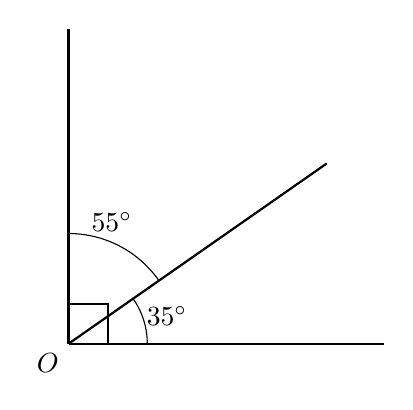
\begin{tikzpicture}[scale=1]
  \coordinate (O) at (0,0);
  \draw[thick] (O) -- (4,0);
  \draw[thick] (O) -- (0,4);
  \draw[thick] (0.5,0) -- (0.5,0.5) -- (0,0.5);
  \draw[thick] (O) -- (3.28,2.29);
  \draw (O) ++(0:1) arc (0:35:1);
  \node at (1.25,0.35) {$35^{\circ}$};
  \draw (O) ++(35:1.4) arc (35:90:1.4);
  \node at (0.55,1.55) {$55^{\circ}$};
  \node[below left] at (O) {$O$};
\end{tikzpicture}
\end{center}

\subsection*{Berpelurus: $125^{\circ}$ dan $55^{\circ}$ berjumlah $180^{\circ}$}
Dua sudut berpelurus bila jumlahnya $180^{\circ}$.
Contoh: $180^{\circ} - 125^{\circ} = 55^{\circ}$.
\begin{center}
\begin{tikzpicture}[scale=1]
  \coordinate (O) at (0,0);
  \draw[thick] (O) -- (-4,0);
  \draw[thick] (O) -- (4,0);
  \draw[thick] (O) -- (2.29,3.28);
  \draw (O) ++(0:1) arc (0:55:1);
  \node at (1.2,0.45) {$55^{\circ}$};
  \draw (O) ++(55:1.4) arc (55:180:1.4);
  \node at (-1.1,1.15) {$125^{\circ}$};
  \node[below] at (O) {$O$};
\end{tikzpicture}
\end{center}

\end{document}
